\documentclass{beamer}
\usetheme{Warsaw}
\useinnertheme{circles}
\useoutertheme[subsection=false]{smoothbars}
\usepackage[utf8x]{inputenc}
\usepackage[czech]{babel}
\usepackage[T1]{fontenc}
\usepackage{listings}
\usepackage[normalem]{ulem}
\usepackage{tikz}

\begin{document}

\AtBeginSection[]
{
  \begin{frame}
    \frametitle{Outline}
    \tableofcontents[currentsection]
  \end{frame}
}

\title{Open Source}
\subtitle{The Brave New World}
\author{Petr Baudiš $\langle${\tt pasky@ucw.cz}$\rangle$}
\institute{Stellenboch 2011\\
	\vskip 1ex
	\pgfdeclareimage[height=4ex]{ccbysa}{by-sa.pdf}
	\pgfuseimage{ccbysa}
}
\date{}
\frame{\titlepage}

\section{Introduction}

\subsection{}
\begin{frame}{The Brave New World\dots}
\begin{center}
{\bf Open Source}
\end{center}
\begin{itemize}
\item Open source code
\item Rights to modify and redistribute the code
\item (Obligation to allow others do the same)
\end{itemize}
\begin{center}

\includegraphics[width=2cm]{opensource-rgb.pdf}\hskip 1em

\includegraphics[width=2cm]{heckert_gnu.pdf}\hskip 1em

\includegraphics[width=2cm]{cc.pdf}
\end{center}
\end{frame}

\subsection{}
\begin{frame}{Why? + Contents}
\begin{itemize}
\item You can improve the world!
\item You can improve yourself!
\item Or at least figure out why it doesn't work.
\pause
\vskip 4ex
\item How did it all happen and what's next
\item How to survive in the open source community
\pause
\vskip 4ex
\item Fork me on Github! {\tt https://github.com/pasky/oss-lec} % TODO
\end{itemize}
\end{frame}


\section{The Story of Open Source}

\subsection{}
\begin{frame}{History}
\begin{columns}
\begin{column}{2cm}
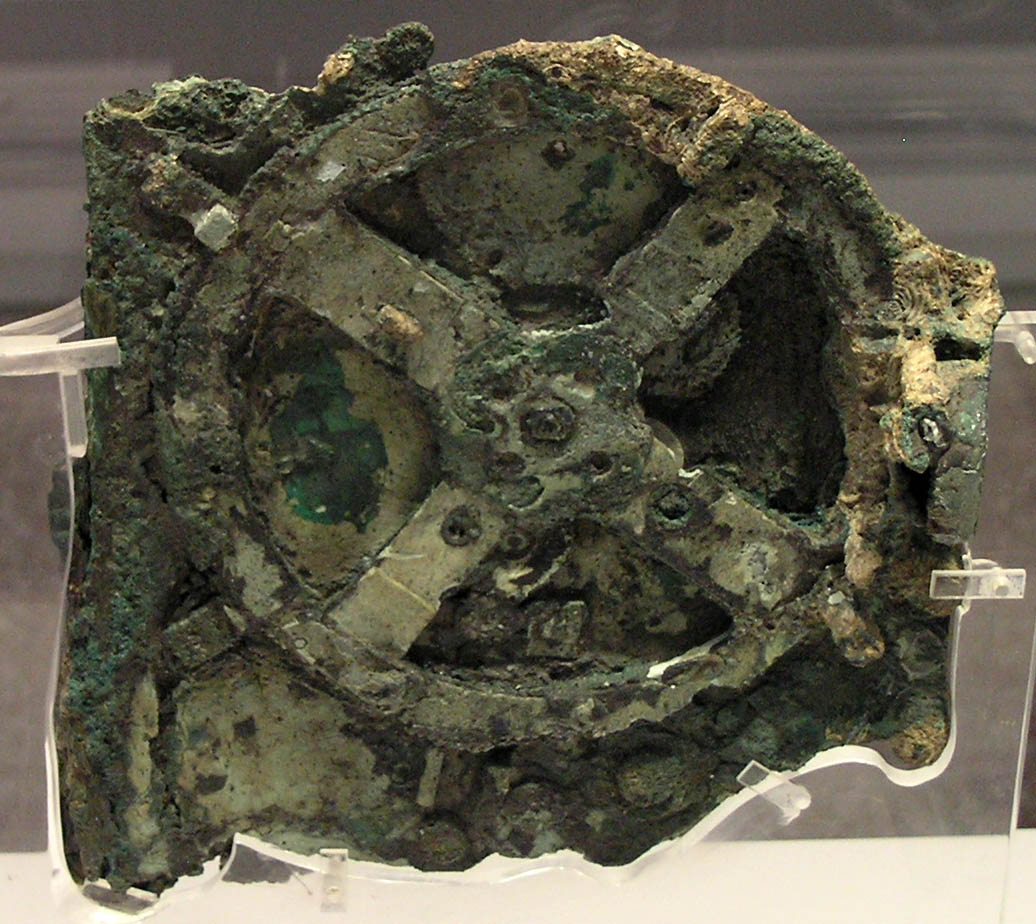
\includegraphics[width=2cm]{antikythera.jpg}
\vskip 3ex
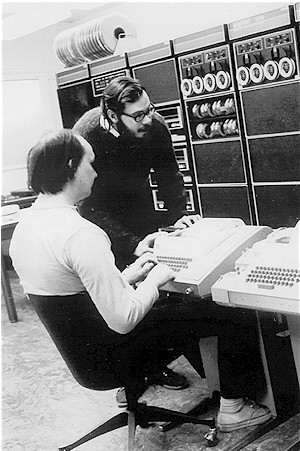
\includegraphics[width=2cm]{pdp11.jpg}
\end{column}
\begin{column}{9cm}
\begin{itemize}
\item Antikythera (150--100 B.C.) --- ancient hi-tech clock, astronomically precise Moon movement, documentation on the case
\item UNIX (1970s A.D.) --- distributed on tapes, of course including the source code
\item Closed source software --- on the rise as the software is decoupled from the hardware
\item 386BSD again opened (rewritten) UNIX code,\\but GNU and Linux appears in the meantime
\end{itemize}
\end{column}
\end{columns}
\end{frame}

\subsection{}
\begin{frame}{The Internet}
\begin{itemize}
\item Communication (USENET, e-mail, IRC) allows world-wide cooperation of programmers (similar to the Wikipedia effect 30 years later)
\item The {\em hacker culture} emerges --- access to the source code \\ is an important attribute
\end{itemize}
\pause
\vskip 2ex
\begin{columns}
\begin{column}{8cm}
\begin{itemize}
\item The internet (based on ARPAnet)\\is completely open system
\item Protocol specs are published as {\em Requests for Comment}, open standards process
\item Jon Postel: ``Be conservative in what you send, liberal in what you accept.''
\end{itemize}
\end{column}
\begin{column}{4cm}
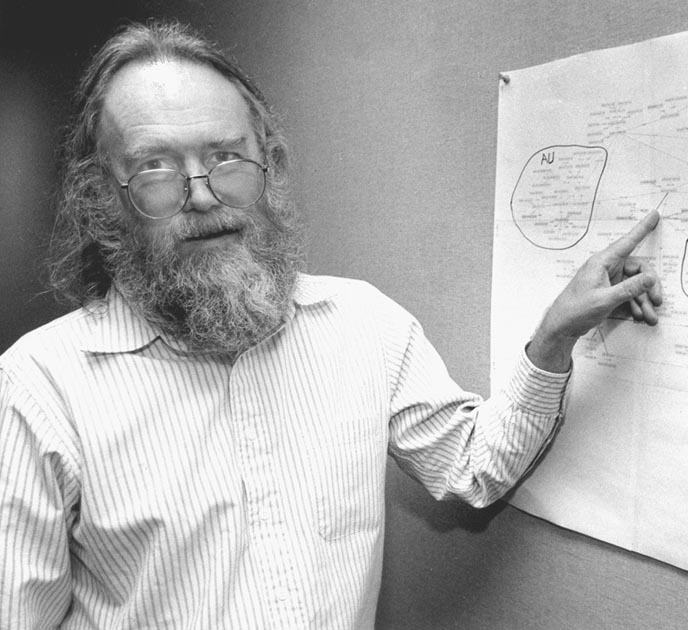
\includegraphics[width=4cm]{Jon_Postel.jpg}
\end{column}
\end{columns}
\end{frame}

\subsection{}
\begin{frame}{The GNU and Free Software Foundation}
\begin{columns}
\begin{column}{9cm}
\begin{itemize}
\item Richard M. Stallman (MIT AI labs):
Can't even tweak the firmware for my printer?
\item Founds GNU in 1983, FSF in 1985
\item {\em Free software} that anyone can modify if he retains this right for others too (``copyleft'').
Unlimited usage and commerce.
\item {\em General Public Licence} (GPL), {\em Lesser GPL}, {\em GFDL}.
\item GNU: Basic tools, text editor, compiler, now also an image editor etc.
\item Kernel by Linus Torvalds $\Rightarrow$ GNU/Linux (but\dots)
\vskip 2ex
\item<2> Non-free software can be even immoral --- {\bf political and social agenda.}
\end{itemize}
\end{column}
\begin{column}{2cm}
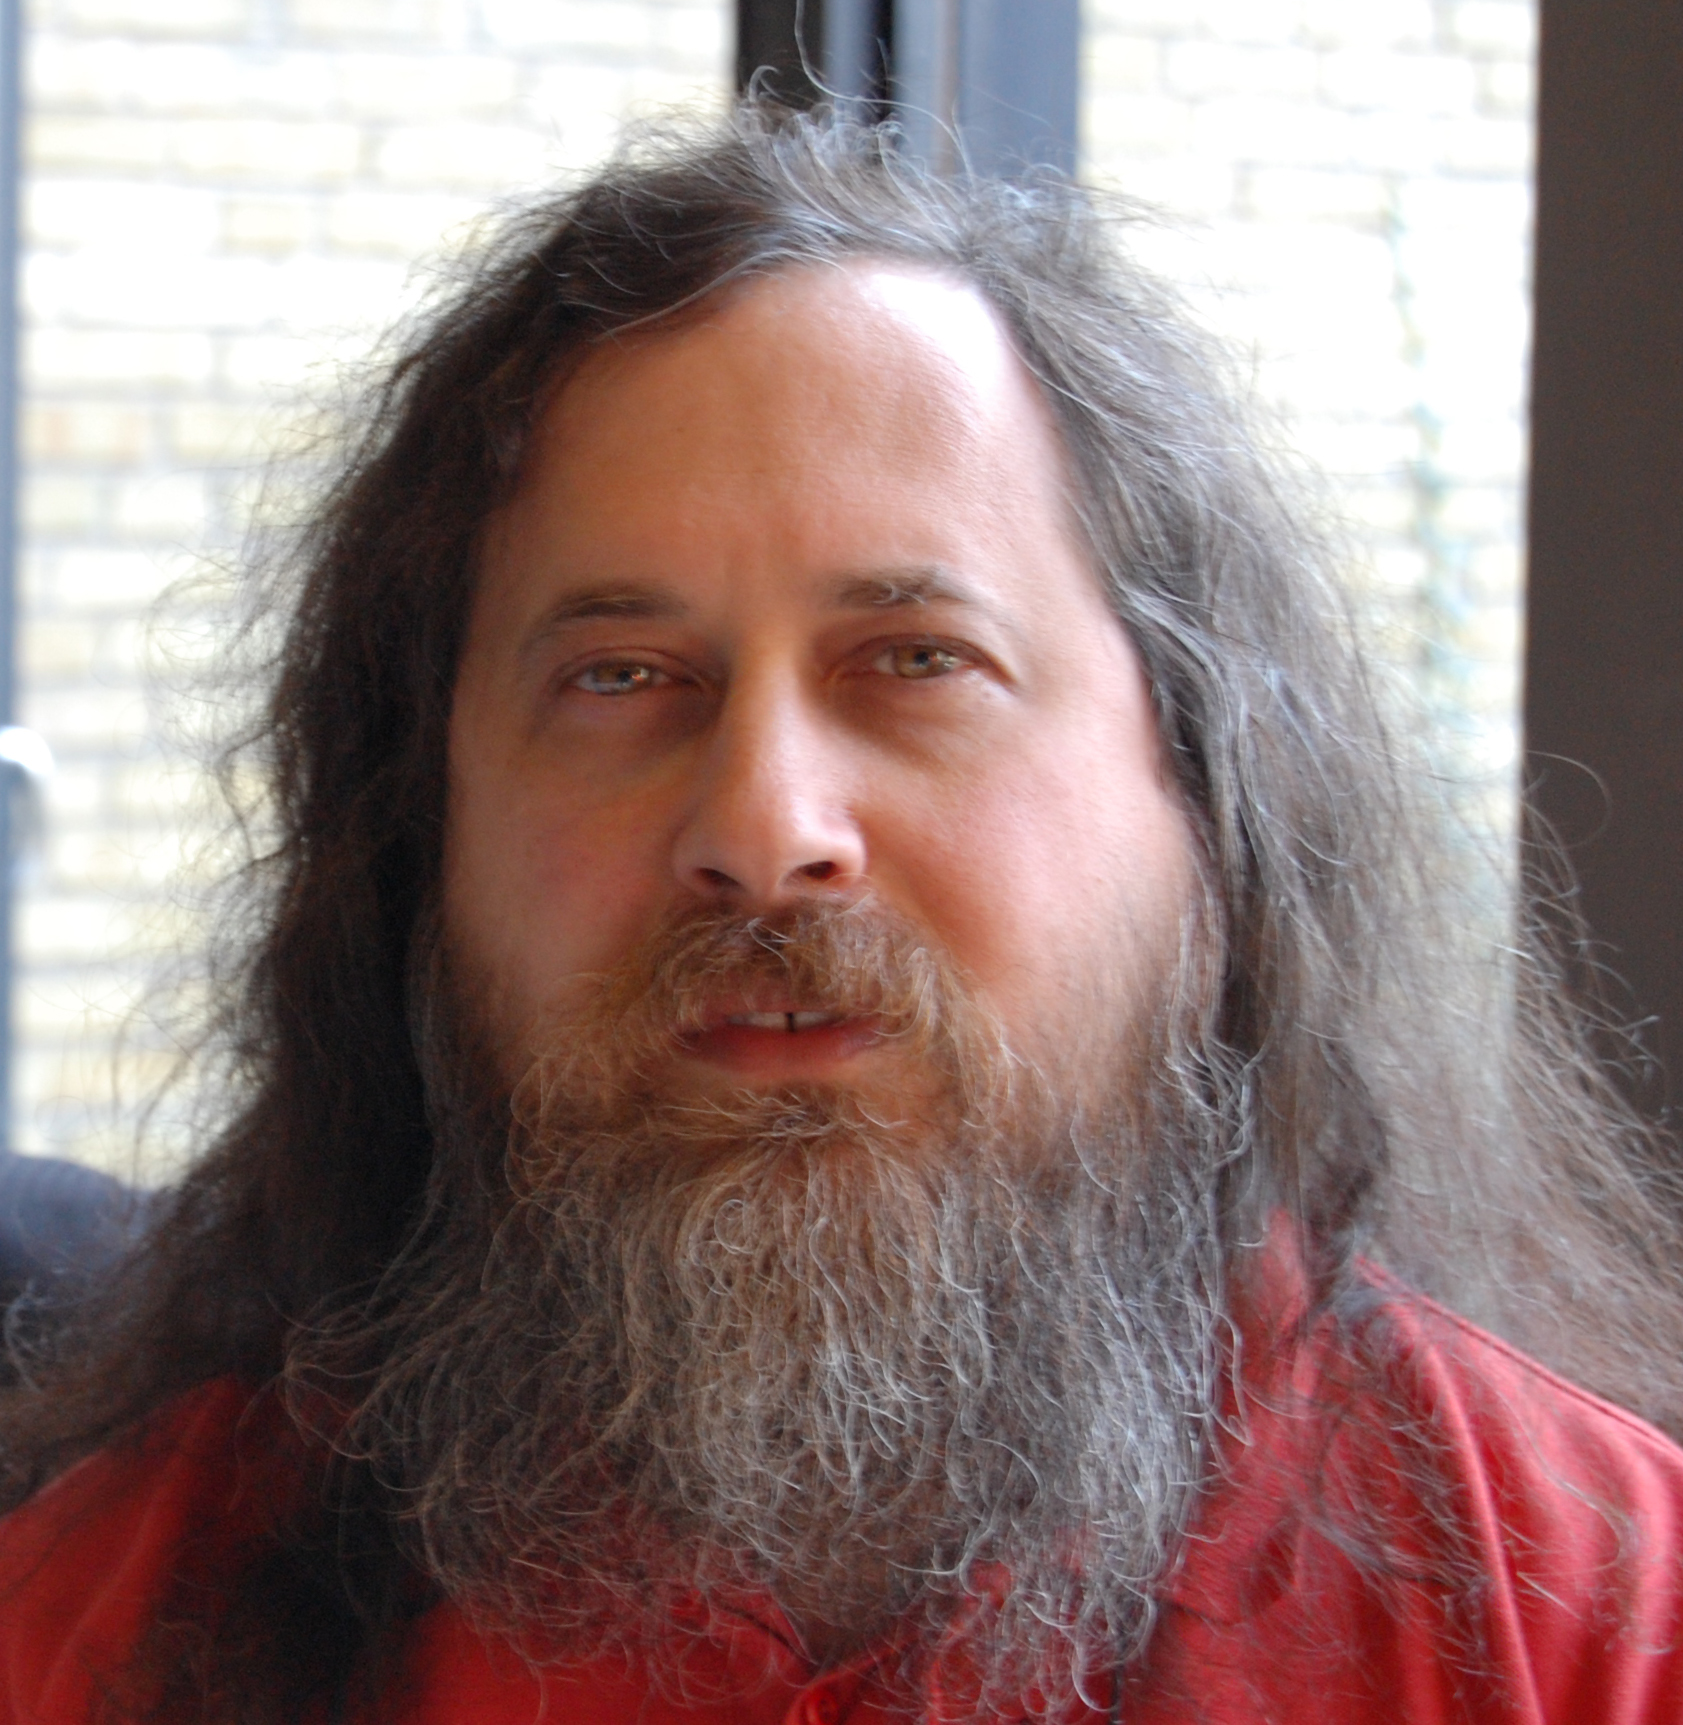
\includegraphics[width=2cm]{rms.jpg}
\vskip 8ex

\includegraphics[width=2cm]{heckert_gnu.pdf}
\end{column}
\end{columns}
\end{frame}

\subsection{}
\begin{frame}{Linus Torvalds, Helsinki}

{\tt \footnotesize
    Hello everybody out there using minix -

    I'm doing a (free) operating system (just a hobby, won't be big and professional like gnu) for 386(486) AT clones. This has been brewing since april, and is starting to get ready. I'd like any feedback on things people like/dislike in minix, as my OS resembles it somewhat (same physical layout of the file-system (due to practical reasons) among other things).

    I've currently ported bash(1.08) and gcc(1.40), and things seem to work. This implies that I'll get something practical within a few months, and I'd like to know what features most people would want. Any suggestions are welcome, but I won't promise I'll implement them :-)

    Linus (torvalds@kruuna.helsinki.fi) \\
    PS. Yes -- it's free of any minix code, and it has a multi-threaded fs. It is NOT portable (uses 386 task switching etc), and it probably never will support anything other than AT-harddisks, as that's all I have :-$($.
}

\end{frame}

\subsection{}
\begin{frame}{Early Linux}
\begin{itemize}
\item {\em Sadly, a kernel by itself gets you nowhere. To get a working system you need a shell, compilers, a library etc. \dots Most of the tools used with linux are GNU software and are under the GNU copyleft.}
\item The Tanenbaum--Torvalds debate:
\begin{itemize}
\item A: {\em \dots{}designing a monolithic kernel in 1991 is
a fundamental error.  Be thankful you are not my student.  You would not
get a high grade for such a design :-) }
\item L: {\em Your job is being a professor and researcher: That's one hell of a
good excuse for some of the brain-damages of minix. }
\item A: {\em I think it is a gross error to design an OS for any specific architecture, since that is not going to be around all that long. }
\item L: {\em An acceptable trade-off, and one that made linux possible in the first place. }
\end{itemize}
\end{itemize}
\end{frame}

\subsection{}
\begin{frame}{Open Source Initiative}
\begin{columns}
\begin{column}{4cm}

\includegraphics[width=4cm]{opensource-rgb.pdf}
\end{column}
\begin{column}{7cm}
\begin{itemize}
\item Free software reduces individual freedom ``for the good of the society'' --- the modified version must be licenced the same way
\item Alternative --- BSD / MIT / X11 etc. licences; short and sweet,\\do anything you want with the sources
\item Open source encompasses these licences as well
\item Open Source Initiative (Bruce Perens, Eric S. Raymond) --- let's stop moralizing and be pragmatic!
\end{itemize}
\end{column}
\end{columns}
\end{frame}

\subsection{}
\begin{frame}{Creative Commons}
\begin{columns}
\begin{column}{4cm}

\includegraphics[width=4cm]{cc.pdf}
\end{column}
\begin{column}{7cm}
\begin{itemize}
\item Software licences don't fit other content well --- or other blueprints
\item Easy to understand, few variants for content creators:
\begin{itemize}
\item BY (attribution)
\item NC (non-commercial)
\item SA (share alike; copyleft again!)
\item ND (no derivative works)
\end{itemize}
\item {\em Free culture} --- pictures, music, writings, other creations;\\{\bf Wikipedia} is the ``poster child''
\end{itemize}
\end{column}
\end{columns}
\end{frame}

\subsection{}
\begin{frame}{The Present}
\begin{columns}
\begin{column}{7cm}
\begin{itemize}
\item The Internet relies on OSS from a large part --- both infrastructure and services
\item Linux in a range of embedded devices (routers, MP3 players, Android)
\item Large companies, academia, sometimes home computers
\vskip 2ex
\item Open software common on Windows too (Firefox, VLC, LibreOffice)
\item Not just software: Project Guttenberg, Wikipedia, Thingiverse
\vskip 2ex
\item Software patents, controversial trademarks, web and (A)GPLv3.
\end{itemize}
\end{column}
\begin{column}{4cm}
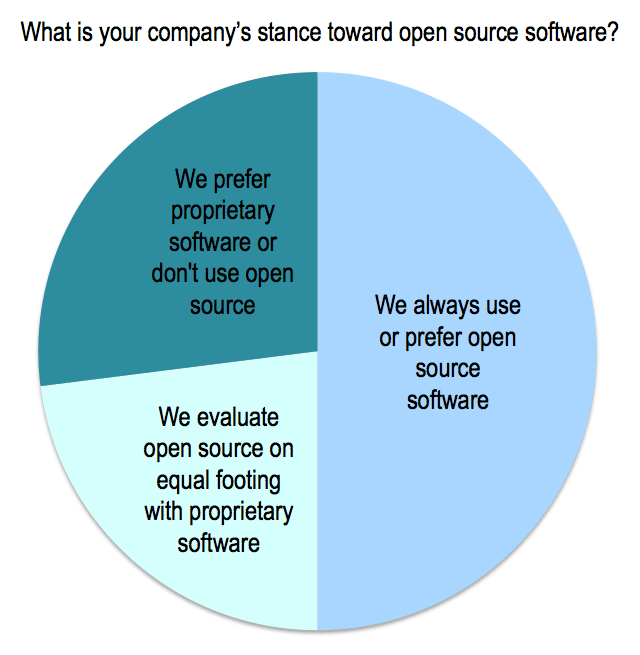
\includegraphics[width=4cm]{Prefer-Or-Prevent.png}
\end{column}
\end{columns}
\end{frame}


\section{Open Source Development}

\subsection{}
\begin{frame}{Project infrastructure}
\begin{itemize}
\item {\em The place where the source code lives}
\item Project homepage --- description, news, \\ download, documentation, development
\item Communication --- mailing list or \\ web forum, wiki, IRC
\item Development --- bugtracker, version control system
\item Index --- distributions, \sout{FreshMeat} FreshCode \\ (\dots, Code Search, Koders.com)
\vskip 3ex
\item Forges: Sourceforge / Savannah, Google Code
\item VCS Hosting: Github / Gitorious, Bitbucket, Launchpad
\end{itemize}
\begin{tikzpicture}[remember picture,overlay]
  \node [xshift=-4.25cm,yshift=-5cm,above right] at (current page.north east)
    {
\includegraphics[width=4cm]{meditate.png}};
\end{tikzpicture}
\end{frame}

\subsection{}
\begin{frame}{A Patching Cookbook}
\begin{itemize}
\item Get the sources. (Web download, {\tt apt-get source}, \dots)
\item Find the right place, grok the conventions,\\keep the coding style. (Doxygen, {\tt HACKING}, \dots)
\item Build it. (Install dependencies, development libraries, \\ {\tt apt-get build-dep}, \dots; {\tt ./configure; make; \\ make install})
\item Document it. Write a testcase if unit testing is used.
\end{itemize}
\end{frame}

\subsection{}
\begin{frame}{A Patch Submission Cookbook}
\begin{itemize}
\item Create a patch or patch series.\\({\tt diff -u} or version control system)
\item Send a patch to the mailing list.\\(Beware whitespace damage, line wrapping.)
% TODO: logo githubu; licence?!
\item Github: Commit changes, fork, push, pull request.
\pause
\vskip 4ex
\item Noone replied in a few days? Resubmit and persist.
\item Respond to comments and bugreports. Ignore rudeness. \\ Be prepared to make major changes in your implementation (but argue first).
\item ``Anyone'' can comment, the maintainer(s) have the last word.
\item Copyright assignment may be required.
\end{itemize}
\end{frame}

\subsection{}
\begin{frame}{Opensourcing a Project Cookbook}
\begin{itemize}
\item Make sure people can easily build and run it.
\item Don't postpone for code cleanup!
\item Pick a licence. When in doubt, GPL or BSD.
\item Write a basic {\tt README} and homepage --- both what it's {\em about}, why is it {\em special} and how to {\em build and use it}. Brief is fine!
\item Advertise in an interest group, expect more work at the beginning.
\item Review, but be liberal in what you accept.
\end{itemize}
\end{frame}

\section{The Future}

\subsection{}
\begin{frame}{The Hackerspaces}
\begin{columns}
\begin{column}{4cm}
%\includegraphics[width=4cm]{HackerspaceLogo}
\vskip 8ex
%\includegraphics[width=4cm]{HackerspacePictureXXX}
\vskip 8ex

\includegraphics[width=4cm]{brmlab.pdf}
\vskip 8ex
%\includegraphics[width=4cm]{BrmlabInterior}
\end{column}
\begin{column}{7cm}
\begin{itemize}
\item The Internet enabled world-wide cooperation of programmers
\item Historically, the academia or large tech companies enabled local cooperation
\item Wider tech accessibility, fragmented community
\pause
\vskip 3ex
\item {\bf Hackerspace} or {\bf makerspace}
\item Independent, community-driven, hacker-run
\item DIY-based, Open Source culture
\item Critical mass, idea polling, base for larger projects
\end{itemize}
\end{column}
\end{columns}
\end{frame}

\subsection{}
\begin{frame}{Open Source Hardware}
\begin{itemize}
% TODO: Pics or it didn't happen!
\item Arduino microcontroller board!
\item Wearable computing, lights and home automation, robots, quadcopters, \dots (hackaday.com)
\item DIY Bio: OpenPCR, simple hacks for DNA analysis, OpenEEG
\item FPGA-based ICs (OpenSPARC, etc.)
\item USRP and GNU Radio --- hack the EM spectrum
\item Global Village Construction Kit
\item RepRap / Maker Bot 3D printing!
\end{itemize}
\end{frame}

\subsection{}
\begin{frame}{Open Source Things}
\begin{itemize}
% TODO: Pics or it didn't happen!
\item 3D printing renaissance in the last 1--2 years
\item Plastic 3D printing --- horizontal layers, ABS or PLA
\item RepRap costs $<10000$ Rands, partially replicable
\pause
\vskip 3ex
\item thingiverse.com: Repository of {\em things} --- download CAD file and print!
\item Fun items --- whistles, action figures, charms, toys
\item Practical accessories like knobs, hooks, doorhandles, simple tools
\item Parts for commercial equipment or DIY projects
\end{itemize}
\end{frame}

\begin{frame}{Thank you!}
\begin{center}
Petr Baudiš $\langle${\tt pasky@ucw.cz}$\rangle$

\vskip 6ex

{\small Faculty of Mathematics and Physics \\ Charles University in Prague}

\vskip 3ex


\includegraphics[width=5cm]{brmlab.pdf}
\end{center}
\end{frame}

\end{document}
